% !TeX root = ../../main.tex
\section{Economic evaluation \& contracts}

\begin{table}[H]
\centering
\caption{Cost of production for Nitroma, expressed in 2020 USD operating for 6600 hours/year}
\label{Cost_of_production}
\begin{tabular}{llllll}
\hline
\multicolumn{2}{l}{\textbf{BASIS}}                              & \textbf{}                             & \multicolumn{2}{l}{\textbf{CAPITAL COST}}              & \textbf{\$}          \\ \cline{1-2} \cline{4-6} 
Location                                & \multicolumn{2}{l}{Nanjing, China}                            & \multicolumn{2}{l}{ISBL}                               & 8,840,486            \\
Capacity (tonne/year)                   & 1549                  &                                       & \multicolumn{2}{l}{OSBL}                               & 3,536,195            \\
Production (tonne/year)                 & 1291                  &                                       & \multicolumn{2}{l}{Land}                               & 2,920,000            \\
Operating Hours                         & 6600                  &                                       & \multicolumn{2}{l}{Design \& engineering}              & 3,094,170            \\
Operating Rate                          & 83\%                  &                                       & \multicolumn{2}{l}{Contingency}                        & 1,237,668            \\
Year                                    & 2021                  &                                       & \multicolumn{2}{l}{One-off chemicals}                  & 9,315                \\ \cline{6-6} 
                                        &                       &                                       & \multicolumn{2}{l}{\textbf{Total fixed investment}}    & \textbf{19,628,519}  \\
                                        &                       &                                       & \multicolumn{2}{l}{\textbf{Working capital}}           & \textbf{2,944,278}   \\ \cline{6-6} 
                                        &                       &                                       & \multicolumn{2}{l}{\textbf{Total investment}}          & \textbf{22,572,797}  \\
                                        &                       &                                       &                           &                            &                      \\
                                        & \textbf{QUANTITY PER} &                                       &                           &                            & \textbf{UNIT COST}   \\
                                        & TONNE OF              &                                       &                           &                            & \textbf{(\$/tonne}   \\
\textbf{RAW MATERIALS}                  & \textbf{PRODUCT}      & \textbf{}                             & \textbf{PRICE (\$/unit)*} & \textbf{COST (\$)}         & \textbf{of product)} \\ \hline
Toluene                                 & 0.97                  & tonnes                                & 570.00                    & 717,335                    & 556                  \\
Nitric acid                             & 1.24                  & tonnes                                & 270.00                    & 432,894                    & 335                  \\
Methanol                                & 0.27                  & tonnes                                & 280.00                    & 99,132                     & 77                   \\
Hydrogen                                & 0.03                  & tonnes                                & 4750.00                   & 172,423                    & 134                  \\
Formic acid                             & 0.80                  & tonnes                                & 360.00                    & 373,905                    & 290                  \\ \cline{5-6} 
\textbf{Total raw materials}            & \textbf{}             & \textbf{}                             & \textbf{}                 & \textbf{1,795,689}         & \textbf{1,391}       \\
                                        &                       &                                       &                           & \textbf{}                  &                      \\
\textbf{UTILITIES}                      &                       &                                       &                           & \textbf{}                  &                      \\
Cooling water (16oC)                    & 0.56                  & tonnes                                & 0.26                      & 241,946                    & 187                  \\
High-pressure steam (4.3 MPa)           & 0.05                  & tonnes                                & 33.68                     & 2,821,950                  & 2,186                \\
Electricity                             & 6.77                  & kWh                                   & 0.10                      & 1,173,140                  & 909                  \\ \cline{5-6} 
\textbf{Total utilities}                & \textbf{}             & \textbf{}                             & \textbf{}                 & \textbf{4,237,036}         & \textbf{3,282}       \\
                                        &                       &                                       &                           & \textbf{}                  &                      \\
\textbf{CATALYSTS}                      &                       &                                       &                           & \textbf{}                  &                      \\
H-Modernite                             & 0.09                  & kg                                    & 15.00                     & 1,770                      & 1                    \\
Palladium-on-carbon (5\%)               & 0.02                  & kg                                    & 6500.00                   & 178,230                    & 138                  \\
Cobalt (II) phthalocyanine              & 1.75                  & kg                                    & 12.00                     & 27,100                     & 21                   \\
Platinum-on-carbon (5\%)                & 0.27                  & kg                                    & 20300.00                  & 7,001,470                  & 5,423                \\ \cline{5-6} 
\textbf{Total catalysts}                & \textbf{}             & \textbf{}                             & \textbf{}                 & \textbf{7,208,570}         & \textbf{5,584}       \\
\textbf{}                               & \textbf{}             & \textbf{}                             & \textbf{}                 & \textbf{}                  & \textbf{}            \\ \cline{5-6} 
\textbf{TOTAL VARIABLE COSTS}           & \textbf{}             & \textbf{}                             & \textbf{}                 & \textbf{13,241,295}        & \textbf{10,257}      \\
                                        &                       &                                       &                           & \textbf{}                  &                      \\
\textbf{DIRECT FIXED COSTS}             &                       &                                       &                           & \textbf{}                  &                      \\
Operating labour                        & 40.00                 & persons                               &                           & 898,188                    &                      \\
Supervision                             & 0.25                  &                                       &                           & 224,547                    &                      \\
Labour overheads                        & 0.60                  & of operating labour and supervision   &                           & 673,641                    &                      \\
Maintenance                             & 0.05                  & of ISBL                               &                           & 442,024                    &                      \\ \cline{5-6} 
\textbf{Total direct fixed costs}       &                       &                                       &                           & \textbf{2,238,401}         & \textbf{1,734}       \\
                                        &                       &                                       &                           & \textbf{}                  &                      \\ \cline{5-6} 
\textbf{DIRECT CASH COST OF PRODUCTION} &                       &                                       &                           & \textbf{15,479,696}        & \textbf{11,991}      \\
                                        &                       &                                       &                           & \textbf{}                  &                      \\
\textbf{ALLOCATED CASH COSTS}           &                       &                                       &                           & \textbf{}                  &                      \\
General overheads                       & \multirow{2}{*}{0.65} & \multirow{2}{*}{of direct fixed cost} &                           & \multirow{2}{*}{1,454,961} &                      \\
(inc. marketing and R\&D)               &                       &                                       &                           &                            &                      \\
Insurance                               & 0.01                  & of ISBL                               &                           & 88,405                     &                      \\
Tax                                     & 0.15                  &                                       &                           & 1,601,589                  &                      \\ \cline{5-6} 
\textbf{Total allocated costs}          &                       &                                       &                           & \textbf{3,144,955}         & \textbf{2,436}       \\
                                        &                       &                                       &                           & \textbf{}                  &                      \\ \cline{5-6} 
\textbf{TOTAL BARE CASH COST}           &                       &                                       &                           & \textbf{18,624,651}        & \textbf{14,427}      \\
                                        &                       &                                       &                           & \textbf{}                  &                      \\
\textbf{FINANCIAL PROVISION}            &                       &                                       &                           & \textbf{}                  &                      \\
Interest                                & 0.05                  &                                       &                           & \textbf{658,692}           &                      \\
Depreciation                            &                       &                                       &                           & \textbf{1,128,640}         &                      \\
                                        &                       &                                       &                           & \textbf{}                  &                      \\ \cline{5-6} 
\textbf{TOTAL COST OF PRODUCTION}       &                       &                                       &                           & \textbf{20,411,983}        & \textbf{15,811}     
\end{tabular}
\end{table}

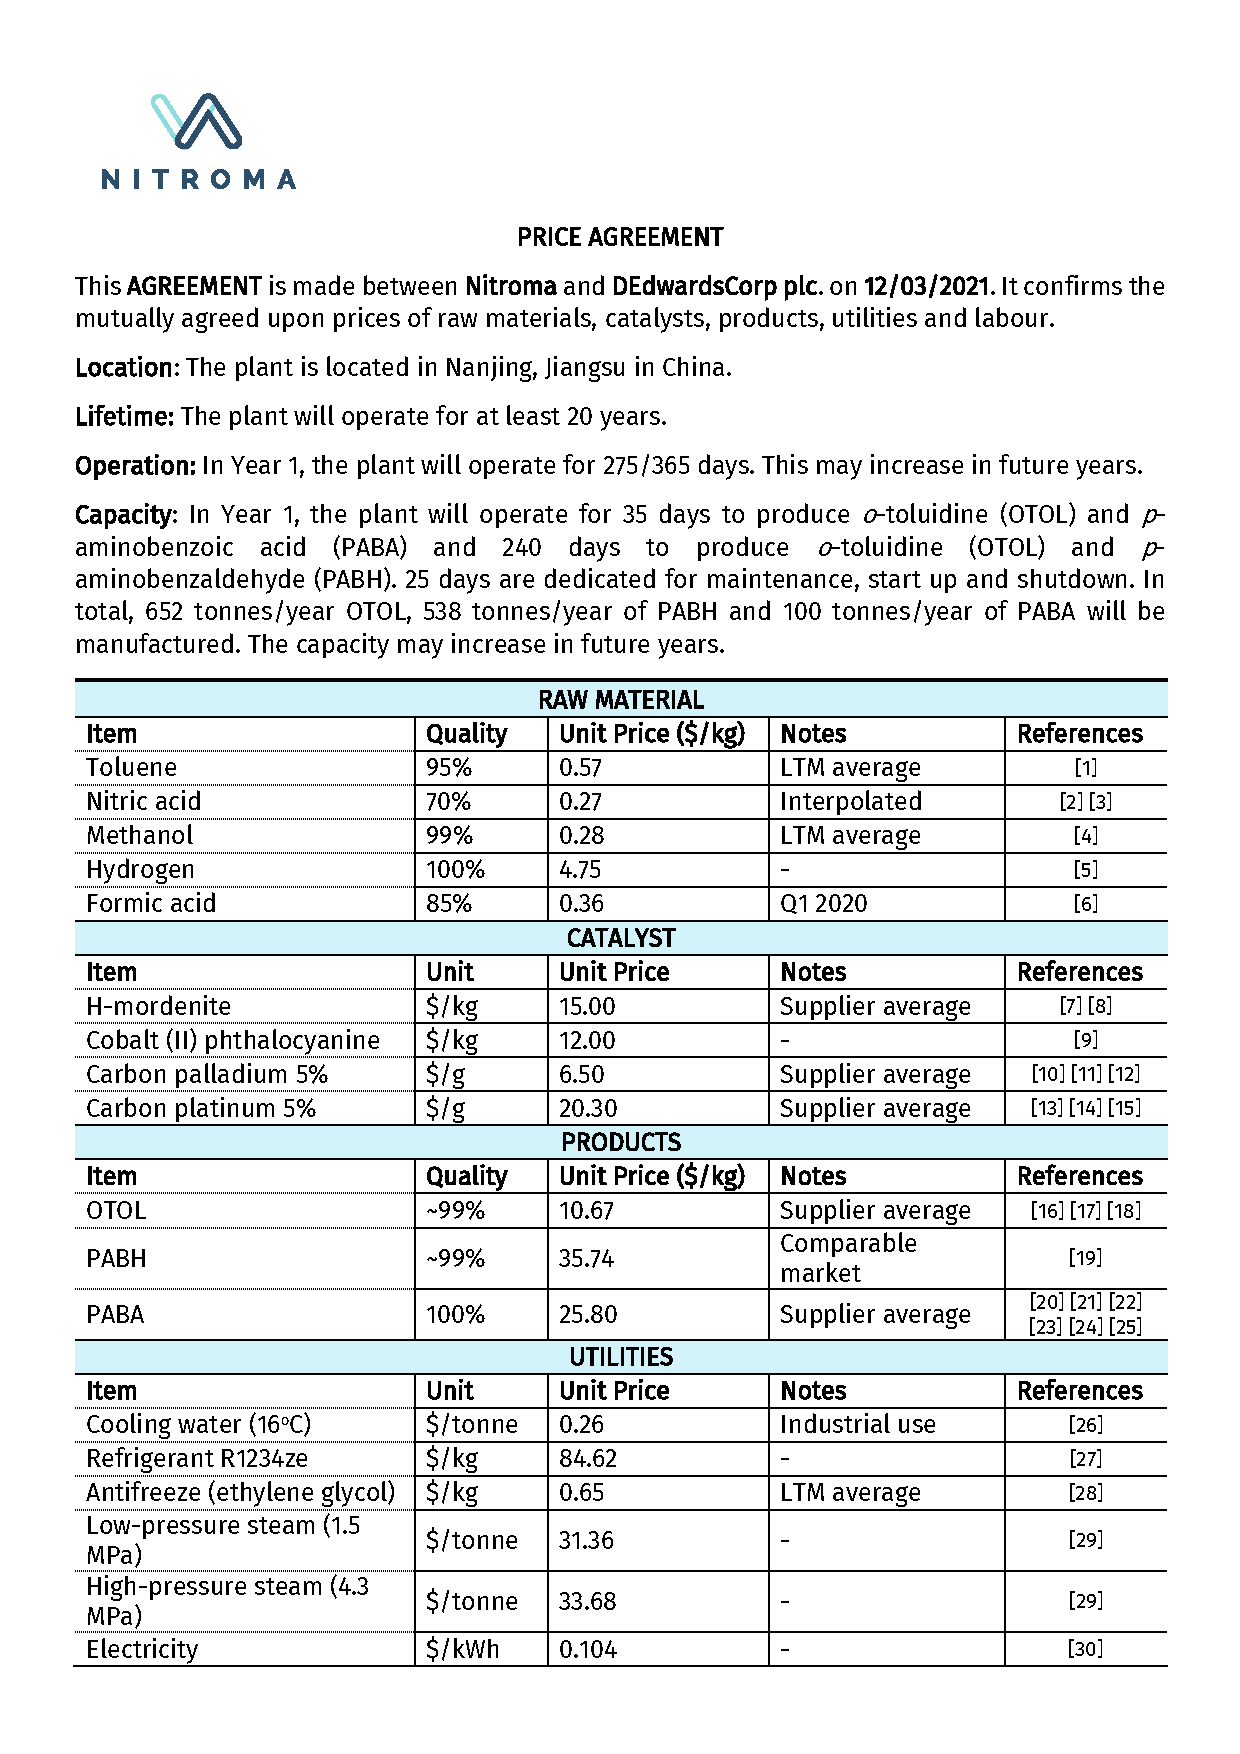
\includepdf[pages=-]{attachments/Price-Agreement-SIGNED_unencrypted.pdf}
